\section{Background}
Maintenance scheduling in industrial predictive maintenance systems is a combinatorial optimization problem that grows exponentially with the number of machines. Given N machines and T discrete time slots, the decision space comprises $T^N$ possible assignments, subject to capacity and assignment constraints. Classical solvers such as Mixed-Integer Linear Programming (MILP) guarantee optimality but face scalability limits for large-scale instances. This section presents quantum and quantum-inspired approaches to maintenance scheduling, evaluating their solution quality, computational cost, and practical feasibility against classical baselines.
Three paradigms are investigated. First, quantum-inspired algorithms that run on classical hardware but exploit heuristics drawn from quantum mechanics. Second, gate-based quantum optimization using the Quantum Approximate Optimization Algorithm (QAOA) executed on IBM Quantum hardware. Third, classical exact optimization via MILP/CBC as the benchmark for optimality.

\section{Problem Formulation}
\subsection{Maintenance Scheduling as Combinatorial Optimization}
The scheduling problem assigns each of N machines to one of T discrete maintenance windows within a planning horizon of H = 72 hours. The slot granularity is s = H / T hours per slot. Each machine i has a priority score $p_i$ in [0, 100] reflecting its failure risk, derived from sensor anomaly detection and damage index estimation by the upstream multi-agent system.
The objective minimizes total scheduling cost:
The optimization objective is defined as:
\begin{equation}
\min_{ \{t_i\}_{i=1}^N } 
\sum_{i=1}^{N} 
\left[
C_{\text{maint}} 
+ C_{\text{risk}} \cdot \frac{p_i}{100} \cdot \frac{t_i}{H}
\right].
\end{equation}

Here, $C_{\text{maint}} = 100$ denotes the fixed maintenance cost, while $C_{\text{risk}} = 1000$ represents the risk-weighted delay penalty. The variable $t_i$ corresponds to the scheduled start time for machine $i$, and $p_i$ indicates its priority score.

This formulation penalises delayed scheduling of high-priority machines. For example, a machine with $p_i = 90$ scheduled at $t_i = 36$ (with $H = 72$) incurs a total cost of:
\begin{equation}
100 + 1000 \cdot 0.9 \cdot \frac{36}{72} = 550,
\end{equation}
whereas scheduling the same machine at $t_i = 0$ results in a cost of only:
\begin{equation}
100.
\end{equation}

\subsection{Constraints}
The feasibility of the optimisation problem is governed by two hard constraints:

\textbf{(1) One-hot assignment constraint.}
Each machine must be assigned to exactly one time slot:
\begin{equation}
\sum_{j=1}^{T} x_{i,j} = 1, \quad \forall i \in \{1, \ldots, N\},
\end{equation}
where $x_{i,j} \in \{0,1\}$ is a binary decision variable indicating whether machine $i$ is scheduled in time slot $j$.

\textbf{(2) Capacity constraint.}
At most $C = 3$ machines can undergo maintenance simultaneously in any time slot:
\begin{equation}
\sum_{i=1}^{N} x_{i,j} \leq C, \quad \forall j \in \{1, \ldots, T\}.
\end{equation}

These constraints reflect practical operational limitations, including maintenance crew availability, spare parts constraints, and safety regulations, all of which restrict the number of concurrent maintenance activities.

\subsection{Time Discretizations}
The number of time slots $T$ is computed adaptively based on the problem parameters:
\begin{equation}
T = \max\!\left(4,\; \left\lceil \frac{N}{C} \right\rceil + \max\!\left(1,\; \left\lfloor \frac{N}{10} \right\rfloor \right) \right).
\end{equation}

This formulation introduces additional slack beyond the minimum required number of slots. At the boundary condition $N = C \cdot T$, the feasible region becomes highly constrained, leading to a near-zero probability of finding valid solutions in the search space. The slack term $\max(1, \lfloor N/10 \rfloor)$ mitigates this degeneracy by expanding the feasible region.

For example, consider $N = 15$ and $C = 3$. The minimum required number of slots is:
\begin{equation}
\left\lceil \frac{15}{3} \right\rceil = 5,
\end{equation}
whereas the adaptive formulation yields:
\begin{equation}
T = 5 + 1 = 6.
\end{equation}

This provides a total capacity of:
\begin{equation}
6 \times 3 = 18,
\end{equation}
which accommodates $15$ machines with a slack ratio of:
\begin{equation}
\frac{18}{15} = 1.2.
\end{equation}

\section{Quadratic Unconstrained Binary Optimization}
Both quantum-inspired and gate-based quantum approaches require the optimisation problem to be formulated as a Quadratic Unconstrained Binary Optimization (QUBO) problem:

\begin{equation}
\min_{\mathbf{x} \in \{0,1\}^n} \; \mathbf{x}^\top \mathbf{Q} \mathbf{x},
\end{equation}

where $\mathbf{x} \in \{0,1\}^n$ is a binary decision vector of dimension $n = N \cdot T$, and $\mathbf{Q} \in \mathbb{R}^{n \times n}$ is a real symmetric matrix.

The QUBO matrix $\mathbf{Q}$ encodes both the objective function and the problem constraints through penalty terms, enabling unconstrained optimization in a quadratic form.

\subsection{Objective Encoding}
The scheduling cost is embedded into the diagonal elements of the QUBO matrix $\mathbf{Q}$. Specifically, for each machine $i \in \{1, \ldots, N\}$ and time slot $j \in \{1, \ldots, T\}$, the diagonal entry is defined as:

\begin{equation}
Q_{(i,j),(i,j)} \; \mathrel{+}= \;
C_{\text{maint}} 
+ C_{\text{risk}} \cdot \frac{p_i}{100} \cdot \frac{j}{T}.
\end{equation}

This construction maps the original linear objective into a quadratic form, leveraging the binary property:
\begin{equation}
x_{i,j}^2 = x_{i,j}, \quad \text{for } x_{i,j} \in \{0,1\}.
\end{equation}

Thus, the contribution of each decision variable $x_{i,j}$ to the objective is encoded directly on the diagonal of $\mathbf{Q}$.

\subsection{Constraint Encoding via Penalty Terms}
Constraints are incorporated into the QUBO formulation through quadratic penalty terms with appropriately calibrated weights.

\textbf{(1) One-hot assignment constraint.}  
The constraint
\begin{equation}
\sum_{j=1}^{T} x_{i,j} = 1
\end{equation}
is enforced using the penalty:
\begin{equation}
\lambda_{\text{assign}} \left( \sum_{j=1}^{T} x_{i,j} - 1 \right)^2.
\end{equation}

Expanding the quadratic term:
\begin{equation}
\left( \sum_{j} x_j - 1 \right)^2 
= - \sum_{j} x_j + 2 \sum_{j<k} x_j x_k + 1,
\end{equation}
where the identity $x_j^2 = x_j$ holds for binary variables.

This yields the following contributions to the QUBO matrix:
\begin{align}
Q_{(i,j),(i,j)} &\;\mathrel{+}= -\lambda_{\text{assign}}, 
&& \text{(diagonal term)} \\
Q_{(i,j),(i,k)} &\;\mathrel{+}= 2\,\lambda_{\text{assign}}, \quad j < k,
&& \text{(off-diagonal, same machine)}.
\end{align}

\textbf{(2) Capacity constraint.}  
To penalize exceeding the capacity limit $C$ for any time slot, pairwise co-assignments are penalized:
\begin{equation}
Q_{(i_1,j),(i_2,j)} \;\mathrel{+}= \frac{\lambda_{\text{cap}}}{C}, 
\quad \forall i_1 \neq i_2,
\end{equation}
for machines assigned to the same time slot $j$.

This discourages assigning more than $C$ machines to the same slot by increasing the energy of infeasible configurations.

\subsection{Penalty Weight Calibration}
To ensure constraint satisfaction, the penalty weights must dominate the objective contributions. Instead of using fixed heuristic values, the penalty coefficients are derived adaptively from the problem parameters.

First, define the maximum possible cost contribution as:
\begin{equation}
C_{\max} = C_{\text{maint}} + C_{\text{risk}} \cdot \max_{i} \left( \frac{p_i}{100} \right).
\end{equation}

The penalty weights are then set as:
\begin{align}
\lambda_{\text{assign}} &= 3 \cdot C_{\max} \cdot T, \\
\lambda_{\text{cap}}    &= 2 \cdot C_{\max}.
\end{align}

The factor of 3 in lambda_assign ensures the one-hot penalty exceeds the maximum possible benefit from any assignment choice, preventing the optimizer from trading constraint violations for lower cost. This data-driven calibration adapts to different problem instances without manual tuning.

\begin{algorithm}[htbp]
\small
\caption{Build QUBO Matrix for Scheduling}
\label{alg:build_qubo}
\begin{algorithmic}[1]
\Require machines with priorities $\{p_i\}_{i=1}^N$, time slots $T$, capacity $C$, costs $(c_{\text{maint}}, c_{\text{risk}})$
\Ensure symmetric QUBO matrix $\mathbf{Q} \in \mathbb{R}^{n \times n}$, where $n = N \cdot T$
\State $n \gets N \cdot T$
\State $\mathbf{Q} \gets \mathbf{0}_{n \times n}$
\Statex \textbf{// Compute data-driven penalty weights}
\State $p_{\max} \gets \max_i \left( \frac{p_i}{100} \right)$
\State $C_{\max} \gets c_{\text{maint}} + c_{\text{risk}} \cdot p_{\max}$
\State $\lambda_{\text{assign}} \gets 3 \cdot C_{\max} \cdot T$
\State $\lambda_{\text{cap}} \gets 2 \cdot C_{\max}$
\Statex \textbf{// Encode scheduling cost on diagonal}
\For{$i = 0$ to $N-1$}
    \For{$j = 0$ to $T-1$}
        \State $k \gets i \cdot T + j$
        \State $Q_{k,k} \gets Q_{k,k} + c_{\text{maint}} + c_{\text{risk}} \cdot \frac{p_i}{100} \cdot \frac{j}{T}$
    \EndFor
\EndFor
\Statex \textbf{// One-hot constraint: $(\sum_j x_{i,j} - 1)^2$}
\For{$i = 0$ to $N-1$}
    \For{$j = 0$ to $T-1$}
        \State $k \gets i \cdot T + j$
        \State $Q_{k,k} \gets Q_{k,k} - \lambda_{\text{assign}}$
    \EndFor
    \For{$j = 0$ to $T-1$}
        \For{$\ell = j+1$ to $T-1$}
            \State $k_1 \gets i \cdot T + j$
            \State $k_2 \gets i \cdot T + \ell$
            \State $Q_{k_1,k_2} \gets Q_{k_1,k_2} + 2 \cdot \lambda_{\text{assign}}$
        \EndFor
    \EndFor
\EndFor
\Statex \textbf{// Capacity constraint: penalise same-slot co-assignment}
\For{$j = 0$ to $T-1$}
    \For{$i_1 = 0$ to $N-1$}
        \For{$i_2 = i_1+1$ to $N-1$}
            \State $k_1 \gets i_1 \cdot T + j$
            \State $k_2 \gets i_2 \cdot T + j$
            \State $Q_{k_1,k_2} \gets Q_{k_1,k_2} + \frac{\lambda_{\text{cap}}}{C}$
        \EndFor
    \EndFor
\EndFor
\Statex \textbf{// Symmetrize matrix}
\State $\mathbf{Q} \gets (\mathbf{Q} + \mathbf{Q}^\top)/2$
\State \Return $\mathbf{Q}$
\end{algorithmic}
\end{algorithm}

\subsection{QUBO to Ising Conversion}
For quantum annealing-based methods (e.g., SQA) and gate-based quantum algorithms (e.g., QAOA), the QUBO formulation is transformed into an equivalent Ising Hamiltonian using the substitution:
\begin{equation}
x_i = \frac{1 + \sigma_i}{2}, \quad \sigma_i \in \{-1, +1\}.
\end{equation}

Under this transformation, the QUBO objective can be expressed as an Ising Hamiltonian:
\begin{equation}
H_{\text{Ising}} = \sum_{i} h_i \, \sigma_i + \sum_{i<j} J_{i,j} \, \sigma_i \sigma_j + \text{offset}.
\end{equation}

The corresponding coefficients are given by:
\begin{align}
h_i &= \frac{Q_{i,i}}{2} + \sum_{j \neq i} \frac{Q_{i,j}}{4}, \\
J_{i,j} &= \frac{Q_{i,j}}{4}, \\
\text{offset} &= \sum_{i} \frac{Q_{i,i}}{4} + \sum_{i<j} \frac{Q_{i,j}}{4}.
\end{align}

\section{Quantum-Inspired Algorithms}
Quantum-inspired algorithms are classical algorithms that incorporate heuristics motivated by quantum mechanical principles. They execute on standard hardware in polynomial time and space, without simulating quantum mechanics. Two algorithms are implemented: the Quantum-Inspired Evolutionary Algorithm (QIEA) and Simulated Quantum Annealing (SQA).

\subsubsection{Quantum-Inspired Evolutionary Algorithm (QIEA)}
QIEA, introduced represents candidate solutions using quantum probability amplitudes rather than classical bitstrings. Each individual in the population is a vector of qubit states:
\begin{equation}
\lvert \psi_i \rangle = \alpha_i \lvert 0 \rangle + \beta_i \lvert 1 \rangle, 
\quad \text{where } \alpha_i^2 + \beta_i^2 = 1.
\end{equation}

The algorithm maintains a population of K such quantum individuals, each encoding a probability distribution over the n-bit decision space.
Observation. At each generation, classical bitstrings are sampled from the amplitude distribution. For each bit i, the observed value is 1 with probability beta$_i^2$ and 0 with probability $alpha_i^2$. This sampling is vectorized for efficiency: probabilities are computed as a K x n matrix, compared against uniform random values, yielding K observed classical solutions per generation.
Evaluation. Each observed bitstring x is evaluated by computing $x^T$ Q x (QUBO energy). The best solution found across all generations is maintained.
Quantum rotation gate update. After evaluation, the Q-gate angles are rotated toward the best-known solution:

\begin{equation}
\Delta \theta = 0.01 \pi \cdot \max\!\left(0.1,\; 1 - \frac{g}{G}\right)
\end{equation}

where g is the current generation and G is the total number of generations. The rotation sign depends on the relationship between the current amplitude bias and the target bit value. This annealing-like schedule reduces the rotation magnitude over time, transitioning from exploration to exploitation. \textbf{Adaptive scaling}. Population size and generation count scale with the problem dimension:
\begin{align}
K &= \max\!\left(20,\; \min\!\left(50,\; \frac{n_{\text{bits}}}{4}\right)\right), \\
G &= \max\!\left(200,\; \min\!\left(400,\; n_{\text{bits}}\right)\right).
\end{align}

This prevents both under-exploration for large problems and wasteful computation for small ones.

% \begin{algorithm}[htbp]
% \small
% \caption{Quantum-Inspired Evolutionary Algorithm (QIEA) for QUBO Optimisation}
% \label{alg:qiea}
% \begin{algorithmic}[1]
% \Require QUBO matrix $\mathbf{Q} \in \mathbb{R}^{n \times n}$, number of variables $n = N \cdot T$, number of machines $N$, number of time slots $T$
% \Ensure Best solution $\mathbf{x}^*$ and energy $E^*$
% \Statex \textbf{// Adaptive parameter scaling}
% \State $K \gets \max\!\left(20,\; \min\!\left(50,\; \left\lfloor \frac{n}{4} \right\rfloor \right)\right)$
% \State $G \gets \max\!\left(200,\; \min\!\left(400,\; n \right)\right)$
% \Statex \textbf{// Initialise quantum population}
% \For{$k = 0$ to $K-1$}
%     \For{$i = 0$ to $n-1$}
%         \State $\alpha_{k,i} \gets \frac{1}{\sqrt{2}}$
%         \State $\beta_{k,i} \gets \frac{1}{\sqrt{2}}$
%     \EndFor
% \EndFor
% \State $\mathbf{x}^* \gets \emptyset$, \quad $E^* \gets +\infty$
% \Statex
% \For{$g = 0$ to $G-1$}
%     \Statex \textbf{// Step 1: Observation}
%     \For{$k = 0$ to $K-1$}
%         \For{$i = 0$ to $n-1$}
%             \State $r \sim \mathcal{U}(0,1)$
%             \State $x_{k,i} \gets 
%             \begin{cases}
%             1, & r < \beta_{k,i}^2 \\
%             0, & \text{otherwise}
%             \end{cases}$
%         \EndFor
%     \EndFor
%     \Statex \textbf{// Step 2: Evaluation}
%     \For{$k = 0$ to $K-1$}
%         \State $E_k \gets \mathbf{x}_k^\top \mathbf{Q} \mathbf{x}_k$
%         \If{$E_k < E^*$}
%             \State $E^* \gets E_k$
%             \State $\mathbf{x}^* \gets \mathbf{x}_k$
%         \EndIf
%     \EndFor
%     \Statex \textbf{// Step 3: Update (Q-gate rotation)}
%     \State $\Delta \theta \gets 0.01\pi \cdot \max\!\left(0.1,\; 1 - \frac{g}{G}\right)$
%     \For{$k = 0$ to $K-1$}
%         \For{$i = 0$ to $n-1$}
%             \If{$x_{k,i} = x^*_i$}
%                 \State \textbf{continue}
%             \EndIf
%             \If{$x^*_i = 1$}
%                 \State $\text{sign} \gets 
%                 \begin{cases}
%                 +1, & \alpha_{k,i} \beta_{k,i} > 0 \\
%                 -1, & \text{otherwise}
%                 \end{cases}$
%             \Else
%                 \State $\text{sign} \gets 
%                 \begin{cases}
%                 -1, & \alpha_{k,i} \beta_{k,i} > 0 \\
%                 +1, & \text{otherwise}
%                 \end{cases}$
%             \EndIf
%             \State $\delta \gets \text{sign} \cdot \Delta \theta$
%             \State $\alpha'_{k,i} \gets \cos(\delta)\,\alpha_{k,i} - \sin(\delta)\,\beta_{k,i}$
%             \State $\beta'_{k,i} \gets \sin(\delta)\,\alpha_{k,i} + \cos(\delta)\,\beta_{k,i}$
%             \State $\alpha_{k,i} \gets \alpha'_{k,i}$
%             \State $\beta_{k,i} \gets \beta'_{k,i}$
%         \EndFor
%     \EndFor
% \EndFor
% \State \Return $\mathbf{x}^*, E^*$
% \end{algorithmic}
% \end{algorithm}

The rotation gate (lines 45–49) is the core quantum-inspired mechanism. Unlike classical genetic algorithms that rely on crossover and mutation, QIEA evolves the probability distribution over solutions. The annealing schedule on Δθ (line 34) ensures broad exploration in early generations (large rotations) and fine-tuning in later generations (small rotations), analogous to the temperature schedule in simulated annealing but operating in the amplitude space.

\section{Simulated Quantum Annealing (SQA)}
SQA simulates quantum annealing using path-integral Monte Carlo. The quantum system with transverse field is mapped to a classical system with an additional (imaginary time) dimension via the Suzuki-Trotter decomposition. The algorithm maintains M = 16 classical replicas (Trotter slices) coupled by an inter-replica interaction:

\begin{equation}
J_{\perp} = -\frac{T_{\text{phys}}}{2} \, \ln\!\left( \tanh\!\left( \frac{\Gamma}{M \, T_{\text{phys}}} \right) \right)
\end{equation}

where Gamma is the transverse field strength and $T_phys$ is the physical temperature.

\textbf{Annealing schedule.} The transverse field Gamma decreases linearly from $Gamma_start$ = 5.0 to $Gamma_end$ = 0.01 over S sweeps. At each sweep, single-spin Metropolis updates are proposed for each spin in each replica. The acceptance criterion accounts for both the problem Hamiltonian energy change and the inter-replica coupling:

\begin{equation}
\Delta E = 2 \, \sigma_i \left[
h_i + \sum_{j} J_{i,j} \, \sigma_j + J_{\perp} \left( \sigma_i^{k-1} + \sigma_i^{k+1} \right)
\right]
\end{equation}

where $sigma_i^{k-1}$ and $sigma_i^{k+1}$ are the spin values in adjacent replicas. The flip is accepted if $Delta_E$ < 0 or with probability $exp(-Delta_E / T_phys)$. \textbf{Sweep scaling}. The number of sweeps adapts to problem size:

\begin{equation}
S = \min\!\left(500,\; \max\!\left(200,\; \frac{500 \cdot 20}{n_{\text{bits}}}\right)\right)
\end{equation}

This caps computation time for large instances while maintaining sufficient sampling for small ones.

The key distinction between SQA and classical simulated annealing lies in the inter-replica coupling term (lines 30–32). The M replicas interact through $J_⊥$, which encodes the effect of quantum tunneling in the Suzuki-Trotter decomposition. When Γ is large, $J_⊥$ is strong and replicas are tightly coupled (high quantum fluctuations); as Γ → 0, $J_⊥$ → 0 and replicas decouple, each converging independently to a classical minimum. The random permutation at line 19 prevents systematic bias in the sweep order.

\section{Gate-Based Quantum Optimization (QAOA)}
\subsection{QAOA with XY Ring Mixer}
The Quantum Approximate Optimization Algorithm (Farhi et al., 2014) constructs a parameterized quantum circuit that alternates between a problem unitary and a mixing unitary. The standard QAOA uses a transverse-field mixer (sum of X gates), which does not respect the one-hot constraint. Following Hadfield et al. (2019), we employ an XY ring mixer that structurally preserves the Hamming weight within each machine's qubit block.

% \begin{algorithm}[htbp]
% \small
% \caption{QAOA with XY Mixer for Scheduling}
% \label{alg:qaoa_xy}
% \begin{algorithmic}[1]
% \Require local fields $\mathbf{h}$, couplings $\mathbf{J}$, machines $N$, time slots $T$, layers $p$, restarts $R$, max iterations $I$
% \Ensure best feasible solution $\mathbf{x}^*$ and cost $C^*$
% \State $n \gets N \cdot T$
% \State $\text{dim} \gets 2^n$
% \Statex \textbf{// Precompute Ising Hamiltonian diagonal}
% \For{$z = 0$ to $\text{dim}-1$}
%     \State $\boldsymbol{\sigma} \gets \text{spin\_vector}(z, n)$
%     \State $H_{\text{diag}}[z] \gets \sum_i h_i \sigma_i + \sum_{i<j} J_{i,j} \sigma_i \sigma_j$
% \EndFor
% \Statex \textbf{// Initial state: one-hot per machine}
% \State $\lvert \psi_{\text{init}} \rangle \gets \bigotimes_{m=1}^{N} \lvert 10\ldots 0 \rangle$
% \State $\gamma^* \gets \emptyset$, \quad $\boldsymbol{\beta}^* \gets \emptyset$, \quad $C^* \gets +\infty$
% \Statex
% \For{$r = 0$ to $R-1$}
%     \State $(\boldsymbol{\gamma}_0, \boldsymbol{\beta}_0) \gets \text{random initial angles in } \mathbb{R}^p \times \mathbb{R}^p$
%     \Statex \textbf{// Define cost function}
%     \Function{QAOA\_Cost}{$\boldsymbol{\gamma}, \boldsymbol{\beta}$}
%         \State $\lvert \psi \rangle \gets \lvert \psi_{\text{init}} \rangle$
%         \For{$\ell = 0$ to $p-1$}
%             \State $\lvert \psi \rangle \gets e^{-i \gamma_\ell H_{\text{diag}}} \lvert \psi \rangle$
%             \For{$m = 0$ to $N-1$}
%                 \For{$t = 0$ to $T-1$}
%                     \State $q_a \gets m \cdot T + t$
%                     \State $q_b \gets m \cdot T + (t+1) \bmod T$
%                     \State Apply XY($\beta_\ell$) on $(q_a, q_b)$:
%                     \Statex \hspace{2em}
%                     $\lvert 01 \rangle \rightarrow \cos(\beta_\ell)\lvert 01 \rangle - i\sin(\beta_\ell)\lvert 10 \rangle$
%                     \Statex \hspace{2em}
%                     $\lvert 10 \rangle \rightarrow -i\sin(\beta_\ell)\lvert 01 \rangle + \cos(\beta_\ell)\lvert 10 \rangle$
%                 \EndFor
%             \EndFor
%         \EndFor
%         \State \Return $\sum_z |\langle z | \psi \rangle|^2 \cdot H_{\text{diag}}[z]$
%     \EndFunction
%     \State $(\boldsymbol{\gamma}_{\text{opt}}, \boldsymbol{\beta}_{\text{opt}}) \gets \text{COBYLA}(\text{QAOA\_Cost}, (\boldsymbol{\gamma}_0, \boldsymbol{\beta}_0), I)$
%     \If{$\text{QAOA\_Cost}(\boldsymbol{\gamma}_{\text{opt}}, \boldsymbol{\beta}_{\text{opt}}) < C^*$}
%         \State $C^* \gets \text{QAOA\_Cost}(\boldsymbol{\gamma}_{\text{opt}}, \boldsymbol{\beta}_{\text{opt}})$
%         \State $\boldsymbol{\gamma}^* \gets \boldsymbol{\gamma}_{\text{opt}}$
%         \State $\boldsymbol{\beta}^* \gets \boldsymbol{\beta}_{\text{opt}}$
%     \EndIf
% \EndFor
% \Statex \textbf{// Sampling best solution}
% \State $\lvert \psi_{\text{final}} \rangle \gets \text{QAOA}(\boldsymbol{\gamma}^*, \boldsymbol{\beta}^*)$
% \State $p(z) \gets |\langle z | \psi_{\text{final}} \rangle|^2$
% \State $\mathbf{x}^* \gets \emptyset$, \quad $\text{Cost}^* \gets +\infty$
% \For{top $200$ states $z$ sorted by $p(z)$}
%     \State $\mathbf{x} \gets \text{binary\_vector}(z, n)$
%     \State feasible $\gets$ true
%     \For{$m = 0$ to $N-1$}
%         \If{$\sum_{j=0}^{T-1} x_{mT+j} \neq 1$}
%             \State feasible $\gets$ false
%         \EndIf
%     \EndFor
%     \If{feasible \textbf{and} $\text{PureCost}(\mathbf{x}) < \text{Cost}^*$}
%         \State $\text{Cost}^* \gets \text{PureCost}(\mathbf{x})$
%         \State $\mathbf{x}^* \gets \mathbf{x}$
%     \EndIf
% \EndFor
% \State \Return $\mathbf{x}^*, \text{Cost}^*$
% \end{algorithmic}
% \end{algorithm}

The critical insight in Algorithm \ref{alg:qaoa_xy}  is that the XY ring mixer (lines 28–37) operates within each machine's qubit block, swapping amplitude only between basis states that have the same Hamming weight. Starting from a one-hot initial state (line 11), the mixer can only reach other one-hot configurations, eliminating the need for the one-hot penalty term during the quantum search and preserving feasibility by construction. This contrasts with QIEA and SQA, which must enforce one-hot constraints through penalty terms in the QUBO energy.

\begin{algorithm}[htbp]
\small
\caption{QAOA Hardware Execution Pipeline}
\label{alg:qaoa_hardware}
\begin{algorithmic}[1]
\Require machines $\mathcal{M}$, time slots $T$, API token, quantum backend
\Ensure best feasible solution $\mathbf{x}^*$ and cost $\text{Cost}^*$
\Statex \textbf{// Phase 1: Parameter optimisation on reduced problem}
\State $N_{\text{opt}} \gets \min(N, 4)$
\State $\mathcal{M}_{\text{opt}} \gets \mathcal{M}[0 : N_{\text{opt}}]$
\State $(\mathbf{h}_{\text{opt}}, \mathbf{J}_{\text{opt}}) \gets \text{BuildQUBO} \rightarrow \text{Ising}(\mathcal{M}_{\text{opt}}, T)$
\State $(\boldsymbol{\gamma}^*, \boldsymbol{\beta}^*) \gets \text{QAOA-XY}(\mathbf{h}_{\text{opt}}, \mathbf{J}_{\text{opt}}, N_{\text{opt}}, T, p, \text{restarts}, \text{max\_iter})$
\Statex \textbf{// Phase 2: Build parameterised circuit}
\State $n_{\text{qubits}} \gets N \cdot T$
\State $qc \gets \text{QuantumCircuit}(n_{\text{qubits}})$
\For{$m = 0$ to $N-1$}
    \State $qc.x(m \cdot T)$
\EndFor
\State $(\mathbf{h}_{\text{full}}, \mathbf{J}_{\text{full}}) \gets \text{BuildQUBO} \rightarrow \text{Ising}(\mathcal{M}, T)$
\For{$\ell = 0$ to $p-1$}
    \Statex \textbf{// Problem unitary}
    \For{$i = 0$ to $n_{\text{qubits}}-1$}
        \State $qc.\text{rz}(2 \gamma^*_\ell \, h_{\text{full}}[i],\; i)$
    \EndFor
    \For{all $(i,j)$ with $J_{\text{full}}[i,j] \neq 0$}
        \State $qc.\text{cx}(i, j)$
        \State $qc.\text{rz}(2 \gamma^*_\ell \, J_{\text{full}}[i,j],\; j)$
        \State $qc.\text{cx}(i, j)$
    \EndFor
    \Statex \textbf{// XY ring mixer}
    \For{$m = 0$ to $N-1$}
        \For{$t = 0$ to $T-1$}
            \State $q_a \gets m \cdot T + t$
            \State $q_b \gets m \cdot T + (t+1) \bmod T$
            \State $qc.\text{cx}(q_a, q_b)$
            \State $qc.\text{ry}(2 \beta^*_\ell, q_a)$
            \State $qc.\text{cx}(q_b, q_a)$
            \State $qc.\text{ry}(-2 \beta^*_\ell, q_a)$
            \State $qc.\text{cx}(q_a, q_b)$
        \EndFor
    \EndFor
\EndFor
\State $qc.\text{measure\_all}()$
\Statex \textbf{// Phase 3: Execute on hardware}
\State $qc_t \gets \text{transpile}(qc, \text{backend}, \text{optimization\_level}=3)$
\State job $\gets \text{SamplerV2}(\text{backend}).\text{run}(qc_t, \text{shots}=4096)$
\State counts $\gets \text{job.result}()$
\Statex \textbf{// Phase 4: Decode and select solution}
\State $\mathbf{x}^* \gets \emptyset$, \quad $\text{Cost}^* \gets +\infty$
\For{each $(\text{bitstring}, \text{count})$ in counts}
    \State $\mathbf{x} \gets \text{decode}(\text{bitstring})$
    \If{$\text{is\_one\_hot}(\mathbf{x}, N, T)$ \textbf{and} $\text{is\_capacity\_ok}(\mathbf{x})$}
        \If{$\text{PureCost}(\mathbf{x}) < \text{Cost}^*$}
            \State $\text{Cost}^* \gets \text{PureCost}(\mathbf{x})$
            \State $\mathbf{x}^* \gets \mathbf{x}$
        \EndIf
    \EndIf
\EndFor
\State \Return $\mathbf{x}^*, \text{Cost}^*$
\end{algorithmic}
\end{algorithm}

Algorithm \ref{alg:qaoa_hardware} addresses the key practical challenge of QAOA on NISQ hardware: the variational optimization loop is prohibitively expensive when executed on-device. The parameter transfer strategy (lines 1–5) optimizes angles on a classically simulable sub-problem, then applies them to the full-size circuit. This assumes concentration of QAOA parameters — that optimal angles for small instances generalize to larger instances of the same problem class (Brandao et al., 2018). The transpilation step (line 43) maps the abstract circuit to the hardware's native gate set and qubit connectivity, introducing SWAP gates that increase circuit depth.
Figure 7 illustrates the circuit architecture for a minimal instance (N = 2 machines, T = 4 time options), showing the initial X-gate preparation, alternating problem unitary (RZ/RZZ) and XY ring mixer layers, and final measurement. Each machine's qubits form an independent block within the mixer, preserving one-hot feasibility.

\begin{figure}[htbp]
    \centering
    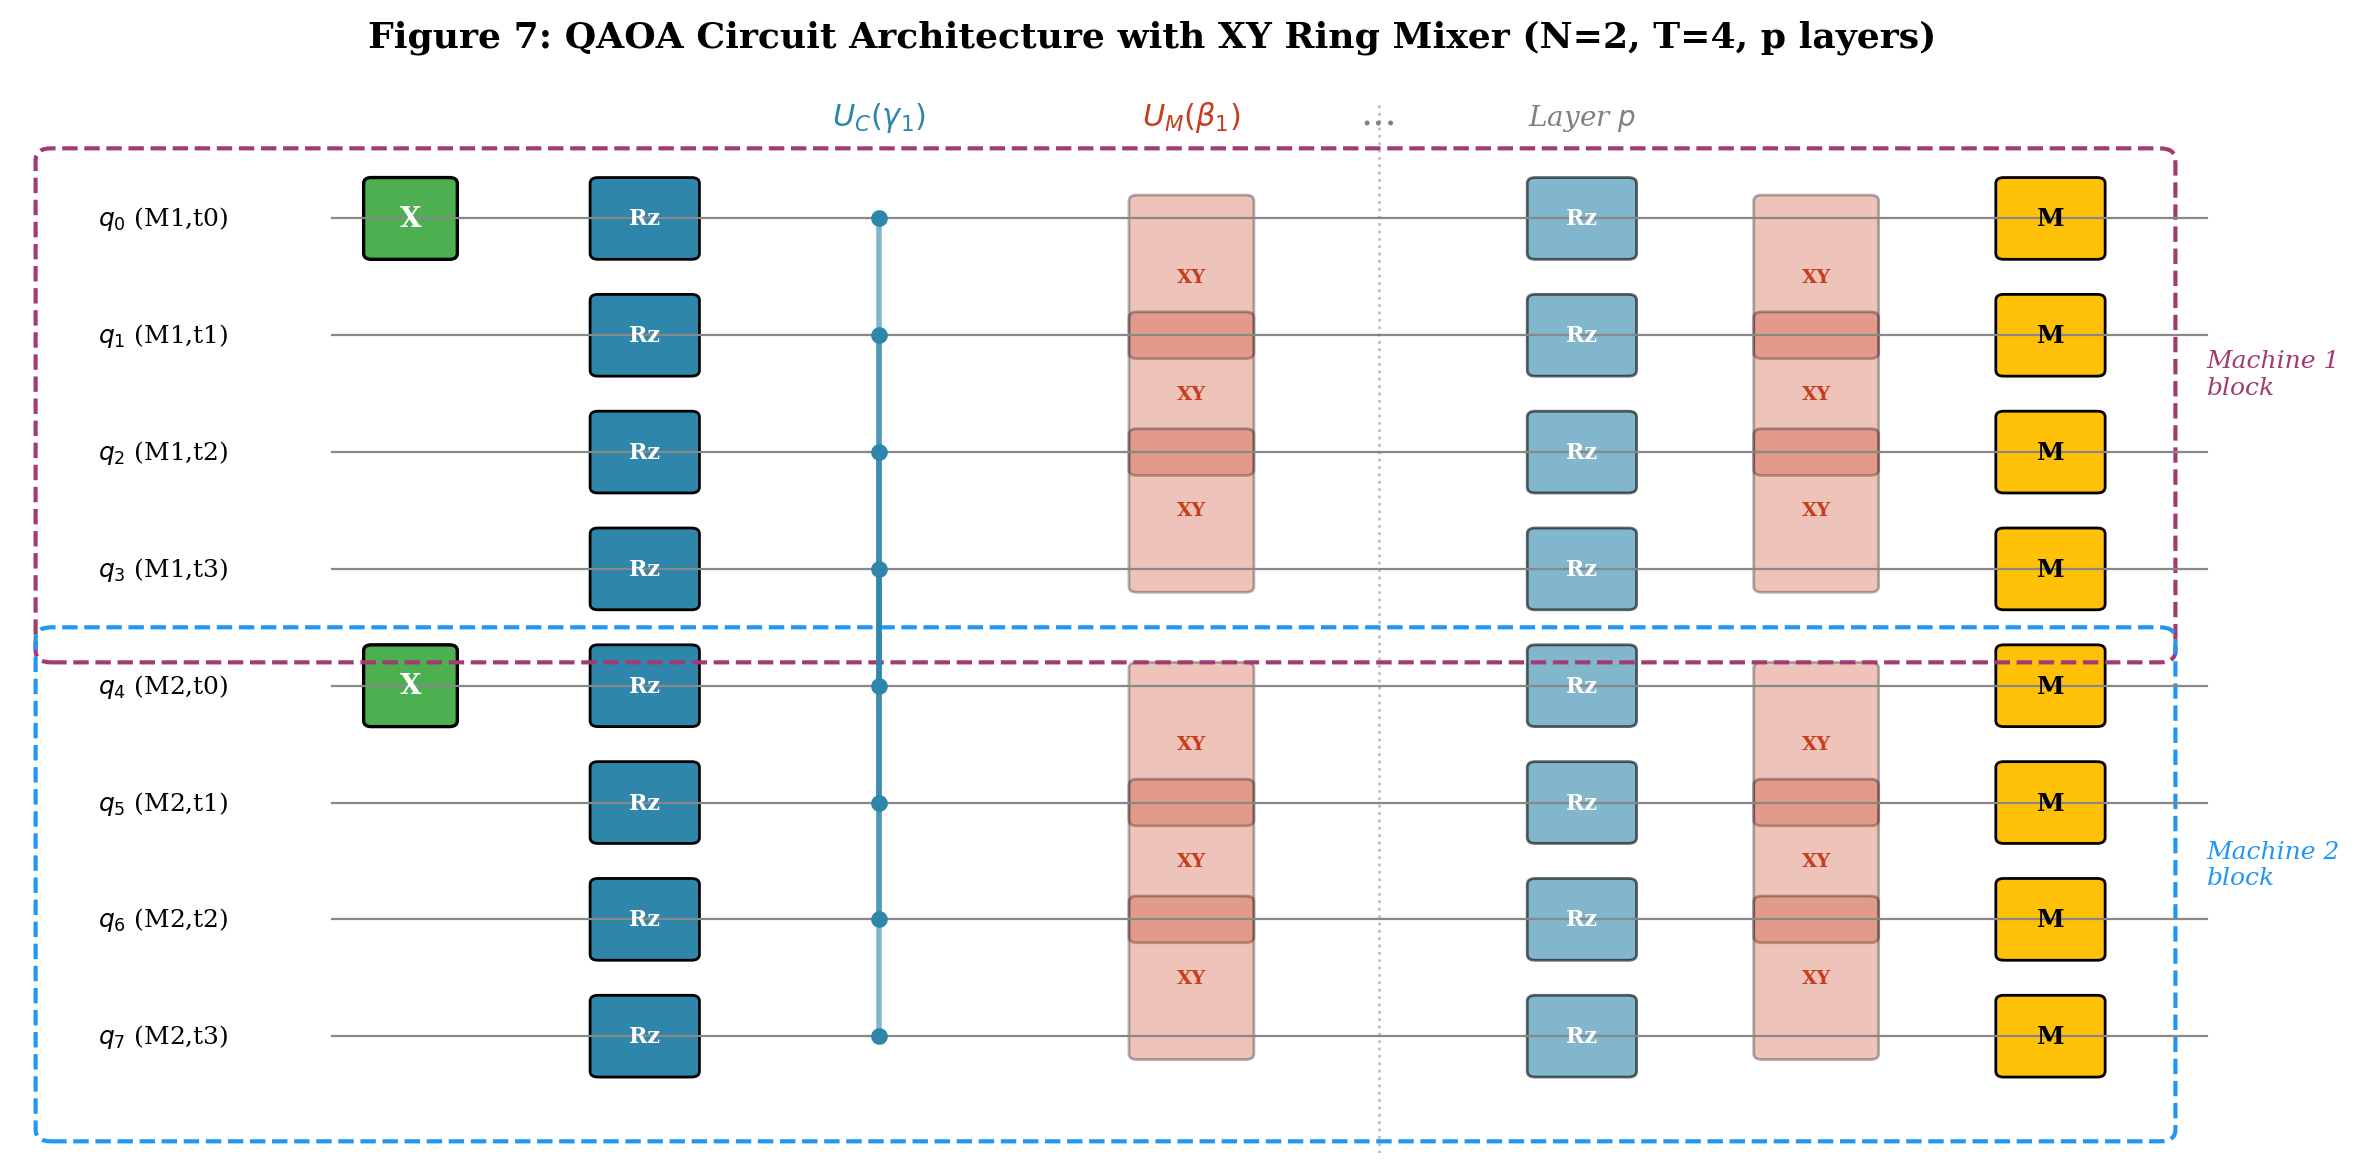
\includegraphics[width=1\textwidth]{figures/images/fig7_qaoa_circuit.png}
    \caption{QAOA circuit architecture for a minimal scheduling instance ($N=2$, $T=4$), showing alternating problem unitary and XY ring mixer layers with final measurement.}
    \label{fig:qaoa-circuit}
\end{figure}

\section{Classical Simulation (State Vector)}
For validation and parameter optimization, the QAOA circuit is simulated using numpy state-vector computation. The state vector has dimension $2^n$, where n = N * T is the number of qubits. This limits classical simulation to approximately N <= 4 machines (16 qubits, 65,536 states) due to exponential memory scaling. Variational parameters $$(gamma_l, beta_l)$ for l = 1, ..., p are optimized using COBYLA with multiple random restarts. The cost function is the expectation value of the problem Hamiltonian:

\begin{equation}
C(\boldsymbol{\gamma}, \boldsymbol{\beta}) 
= \langle \psi(\boldsymbol{\gamma}, \boldsymbol{\beta}) \mid H_C \mid \psi(\boldsymbol{\gamma}, \boldsymbol{\beta}) \rangle
= \sum_{z} \left| \langle z \mid \psi \rangle \right|^2 \, E_z
\end{equation}

After optimization, the state is sampled and the lowest-energy feasible bitstring is selected.

\section{IBM Quantum Hardware Execution}
For problem sizes beyond classical simulation limits, the QAOA circuit is executed on real quantum hardware via IBM Quantum Platform. The implementation targets IBM Heron r2 processors $(ibm_fez, 156 qubits)$.
\textbf{Parameter transfer}. Variational parameters are optimized on a classical simulator using a reduced problem (4 machines), then transferred to the full-size circuit. This avoids expensive on-device optimization loops while providing good initial angles (Brandao et al., 2018). \textbf{Transpilation}. The abstract circuit is transpiled to the hardware's native gate set (CZ, SX, RZ) and qubit connectivity using Qiskit's transpiler at optimization level 3. This step introduces routing overhead: additional SWAP gates to satisfy the hardware's coupling map. \textbf{Execution}. The transpiled circuit is executed using SamplerV2 via Qiskit Runtime. Measurement results (4096 shots) are decoded to bitstrings, checked for feasibility, and the lowest-cost feasible solution is selected.
Noise effects. Hardware noise causes decoherence, reducing solution quality. The estimated circuit fidelity scales as:
\begin{equation}
F_{\text{est}} = (1 - \epsilon_{\text{CZ}})^{n_{\text{CZ}}}
\end{equation}

where $epsilon_CZ$ is approximately 0.004 (CZ gate error rate) and $n_CZ$ is the number of CZ gates after transpilation. For large circuits, this fidelity decays exponentially, establishing a noise-scaling frontier beyond which the output degrades to uniform random noise.

\section{Classical Baseline : MILP / CBC}
The Mixed-Integer Linear Programming formulation serves as the optimality benchmark. To ensure fair comparison, the MILP uses the same T discrete time slots as the quantum approaches, rather than all 72 hourly slots. The formulation is:
\begin{equation}
\begin{aligned}
\min_{\{M_{i,t}\}} \quad 
& \sum_{i,t} \left[
C_{\text{maint}} \, M_{i,t} 
+ C_{\text{risk}} \cdot \frac{p_i}{100} \cdot \frac{t \cdot s}{H} \, M_{i,t}
\right] \\
\text{s.t.} \quad
& \sum_{t} M_{i,t} = 1, \quad \forall i \quad \text{(one-hot)} \\
& \sum_{i} M_{i,t} \leq C, \quad \forall t \quad \text{(capacity)} \\
& M_{i,t} \in \{0,1\}.
\end{aligned}
\end{equation}

where s = H / T is the slot duration in hours. This is solved by the CBC solver (COIN-OR Branch and Cut), which guarantees global optimality for moderate-scale instances.

\section{Experimental Results}
\subsection{Experiment Setup}
All experiments use a common problem generator with deterministic random seeds for reproducibility. Machine priority scores are drawn uniformly from [20, 100], and approximately 30\% of machines are flagged as $risk_state$ = True. The cost parameters are $C_maint$ = 100, $C_risk$ = 1000, with capacity C = 3 and maintenance duration 4 hours.
The pure scheduling cost (without penalty terms) is used as the comparison metric across all methods:

\begin{equation}
\text{Cost}_{\text{pure}} 
= \sum_{i} \left[
C_{\text{maint}} 
+ C_{\text{risk}} \cdot \frac{p_i}{100} \cdot \frac{\text{start}_i}{72}
\right]
\end{equation}

This metric is directly comparable across MILP, quantum-inspired, and quantum methods, as it excludes the QUBO penalty terms that are internal to the quantum formulations.

\subsection{Unified Benchmark (N = 3 - 100}
Table 1 presents results from the unified benchmark comparing all methods on the same problem instances.

\begin{table}[htbp]
\centering
\caption{Unified Benchmark Results}
\label{tab:bmk}
\renewcommand{\arraystretch}{1.2}

\begin{tabularx}{\textwidth}{
c c c c c c c c c
}
\toprule
\textbf{N} & \textbf{n\_bits} & \textbf{MILP Cost} & \textbf{MILP Time} 
& \textbf{QIEA Cost} & \textbf{QIEA Time} & \textbf{QIEA Gap} 
& \textbf{QAOA/sim Cost} & \textbf{QAOA/sim Time} \\
\midrule

3  & 12 & 300.00 & 6 ms     & 300.00 & 35 ms    & 0.0\%  & 300.00 & 15{,}217 ms \\
5  & 20 & 642.50 & 6 ms     & 1{,}046.50 & 50 ms & 62.9\% & --- & --- \\
7  & 28 & 1{,}248.25 & 6 ms & 2{,}252.00 & 75 ms & 80.4\% & --- & --- \\
10 & 50 & 2{,}060.69 & infeasible & 110 ms & --- & --- & --- & --- \\

\bottomrule
\end{tabularx}
\footnotesize
\textit{Note: QAOA/sim is limited to $N \leq 4$ due to state-vector memory constraints. 
Gap is computed as $(\text{Cost}_{\text{method}} - \text{Cost}_{\text{MILP}})/\text{Cost}_{\text{MILP}} \times 100\%$. 
Dashes (---) indicate that the method was not executed at that scale.}

\end{table}

At N = 3, both QIEA and QAOA/sim achieve the exact MILP optimum (gap = 0.0\%), validating the correctness of the QUBO formulation and solver implementations. For larger instances, QAOA simulation becomes infeasible due to $O(2^n)$ memory requirements, while QIEA remains tractable with gaps of 63-80\%. Figure 3 visualizes this comparison across all methods.

\begin{figure}[htbp]
    \centering
    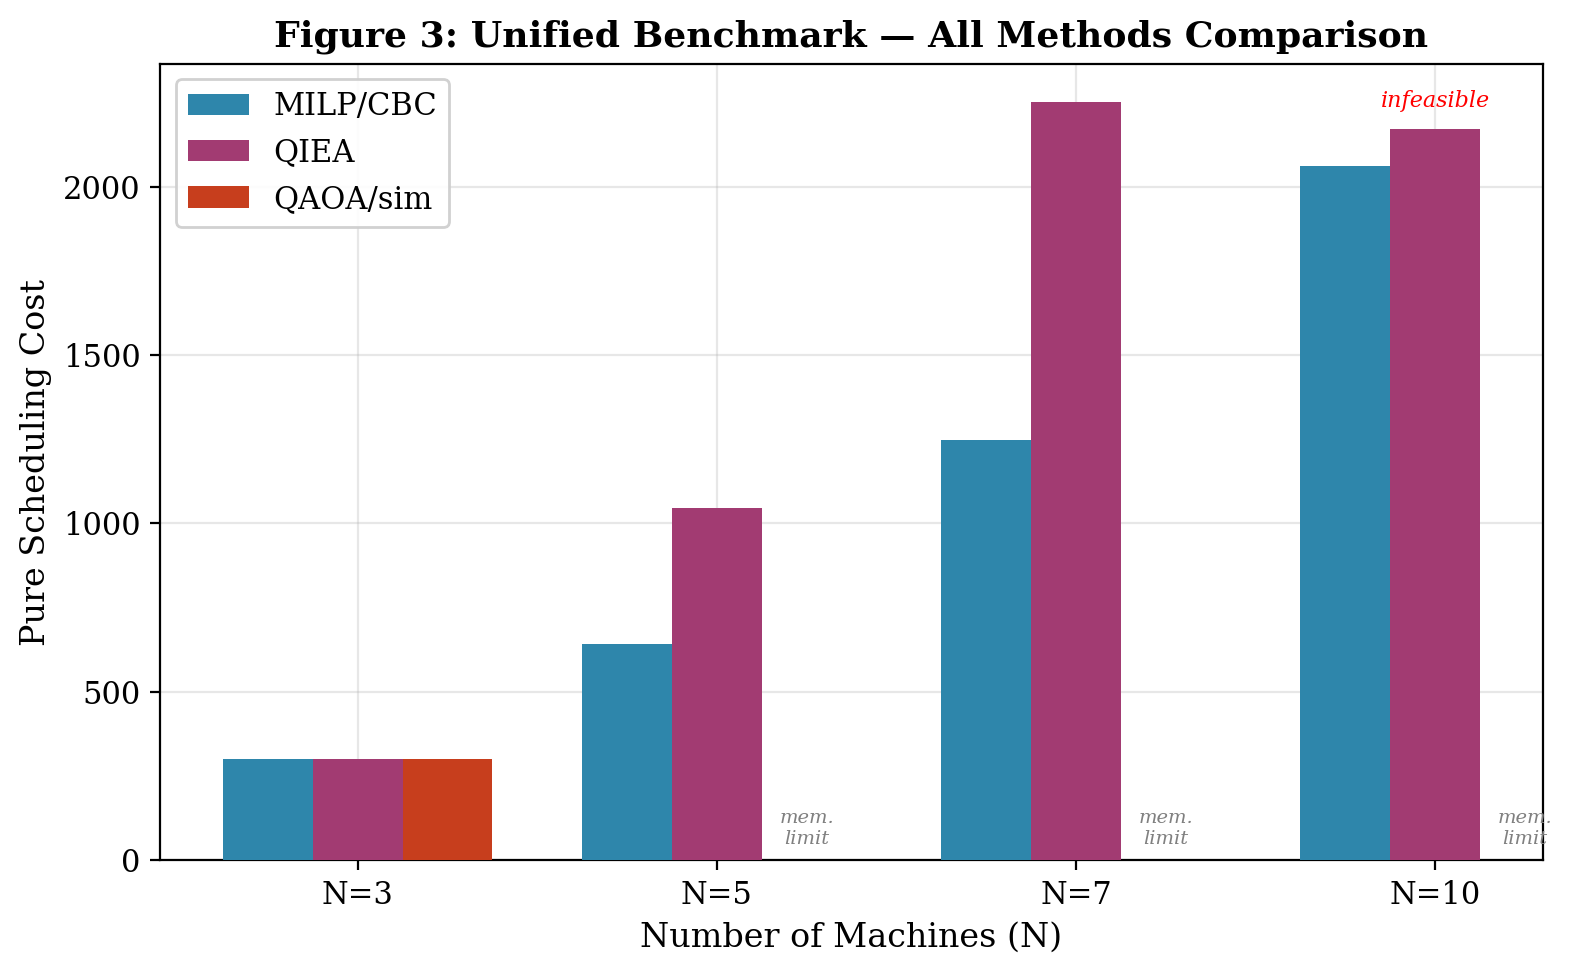
\includegraphics[width=1\textwidth]{figures/images/fig3_unified_benchmark.png}
    \caption{Unified Benchmark - All Methods Comparison.}
    \label{fig:unified-benchmark}
\end{figure}

\subsection{Scaling Benchmark (N = 5 to 30}

Table \ref{tab:scal} presents the extended scaling study comparing MILP, QIEA, and SQA across larger problem instances.

\begin{table}[htbp]
\centering
\caption{Scaling benchmark comparing MILP, QIEA, and SQA across fleet sizes $N=5$ to $N=30$.}
\label{tab:scal}
\renewcommand{\arraystretch}{1.2}

\begin{tabularx}{\textwidth}{
c c c c c c c
}
\toprule
\textbf{N} & \textbf{n\_time\_options} & \textbf{MILP Cost} 
& \textbf{QIEA Cost} & \textbf{QIEA Gap} 
& \textbf{SQA Cost} & \textbf{SQA Gap} \\
\midrule

5  & 4  & 531.67   & 813.25   & 53.0\%  & 1{,}100.75 & 107.0\% \\
10 & 5  & 1{,}303.06 & 2{,}563.14 & 96.7\%  & 3{,}264.11 & 150.5\% \\
15 & 6  & 2{,}180.44 & 4{,}713.17 & 116.2\% & --- & --- \\
20 & 9  & 3{,}221.61 & 7{,}070.89 & 119.5\% & --- & --- \\
25 & 11 & 4{,}489.89 & 7{,}348.25 & 63.7\%  & --- & --- \\
30 & 13 & 6{,}413.56 & 10{,}317.57 & 60.9\% & --- & --- \\

\bottomrule
\end{tabularx}
\footnotesize
\textit{Note: SQA skipped for $N \gt 10$ due to timeout. Gap $= (\text{Cost}_{\text{method}} - \text{Cost}_{\text{MILP}})/\text{Cost}_{\text{MILP}} \times 100\%$. Dashes indicate method not executed at that scale.}

\end{table}

\begin{figure}[htbp]
    \centering

    \begin{subfigure}[t]{0.48\textwidth}
        \centering
        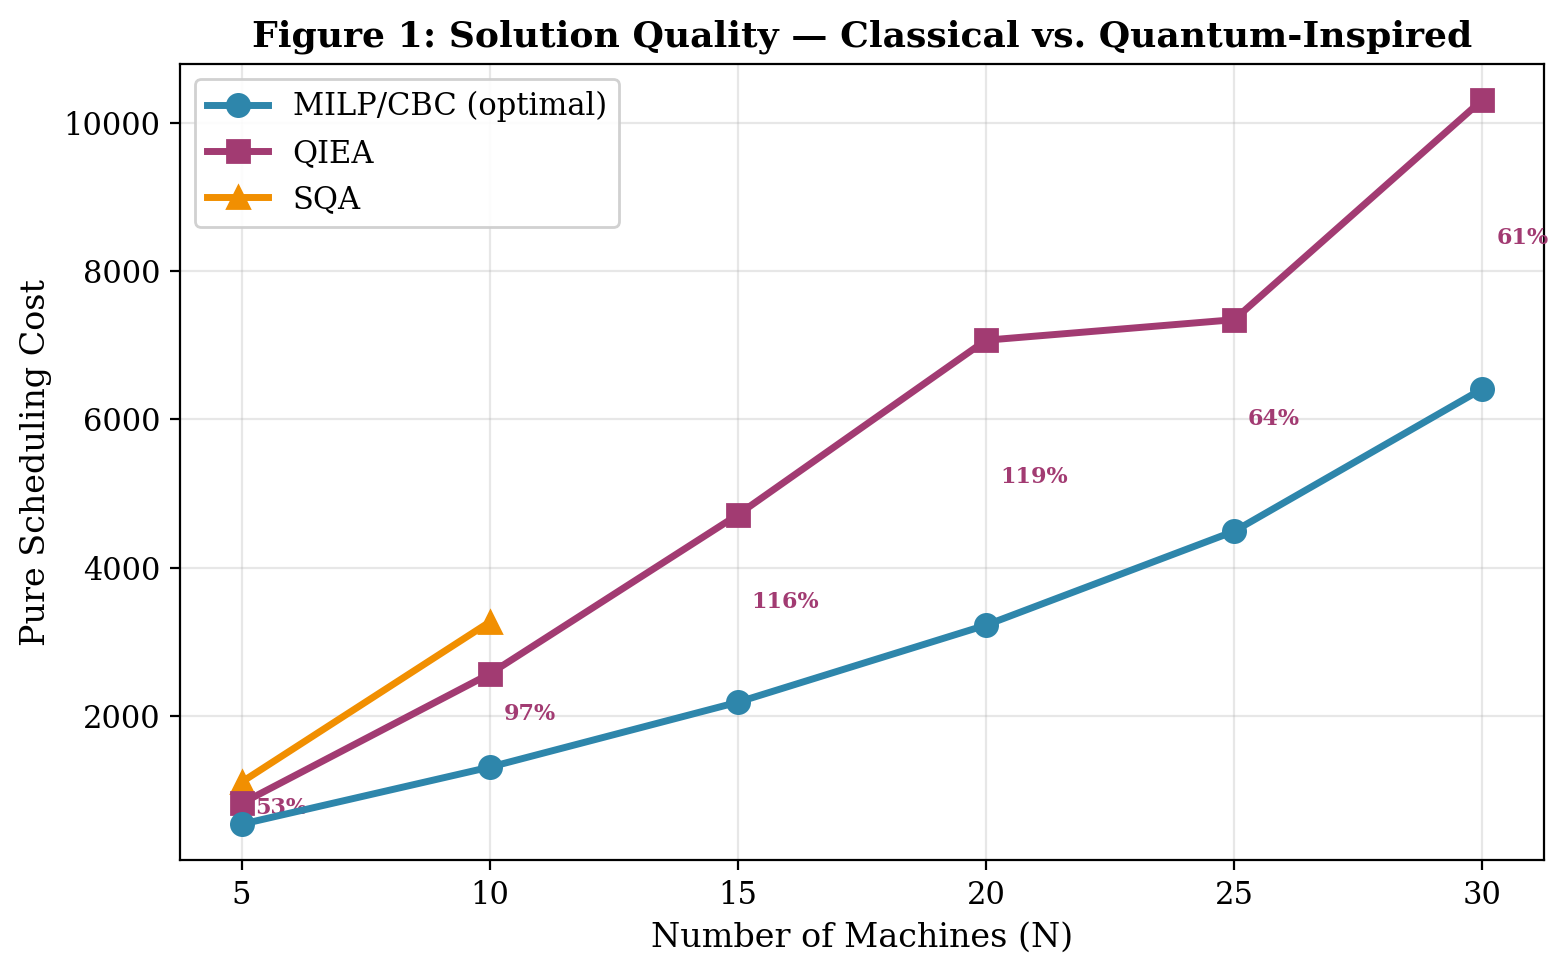
\includegraphics[width=\textwidth]{figures/images/fig1_solution_quality_scaling.png}
        \caption{Solution quality (total cost) vs. fleet size $N$ for MILP, QIEA, and SQA.}
        \label{fig:quality_scaling}
    \end{subfigure}
    \hfill
    \begin{subfigure}[t]{0.48\textwidth}
        \centering
        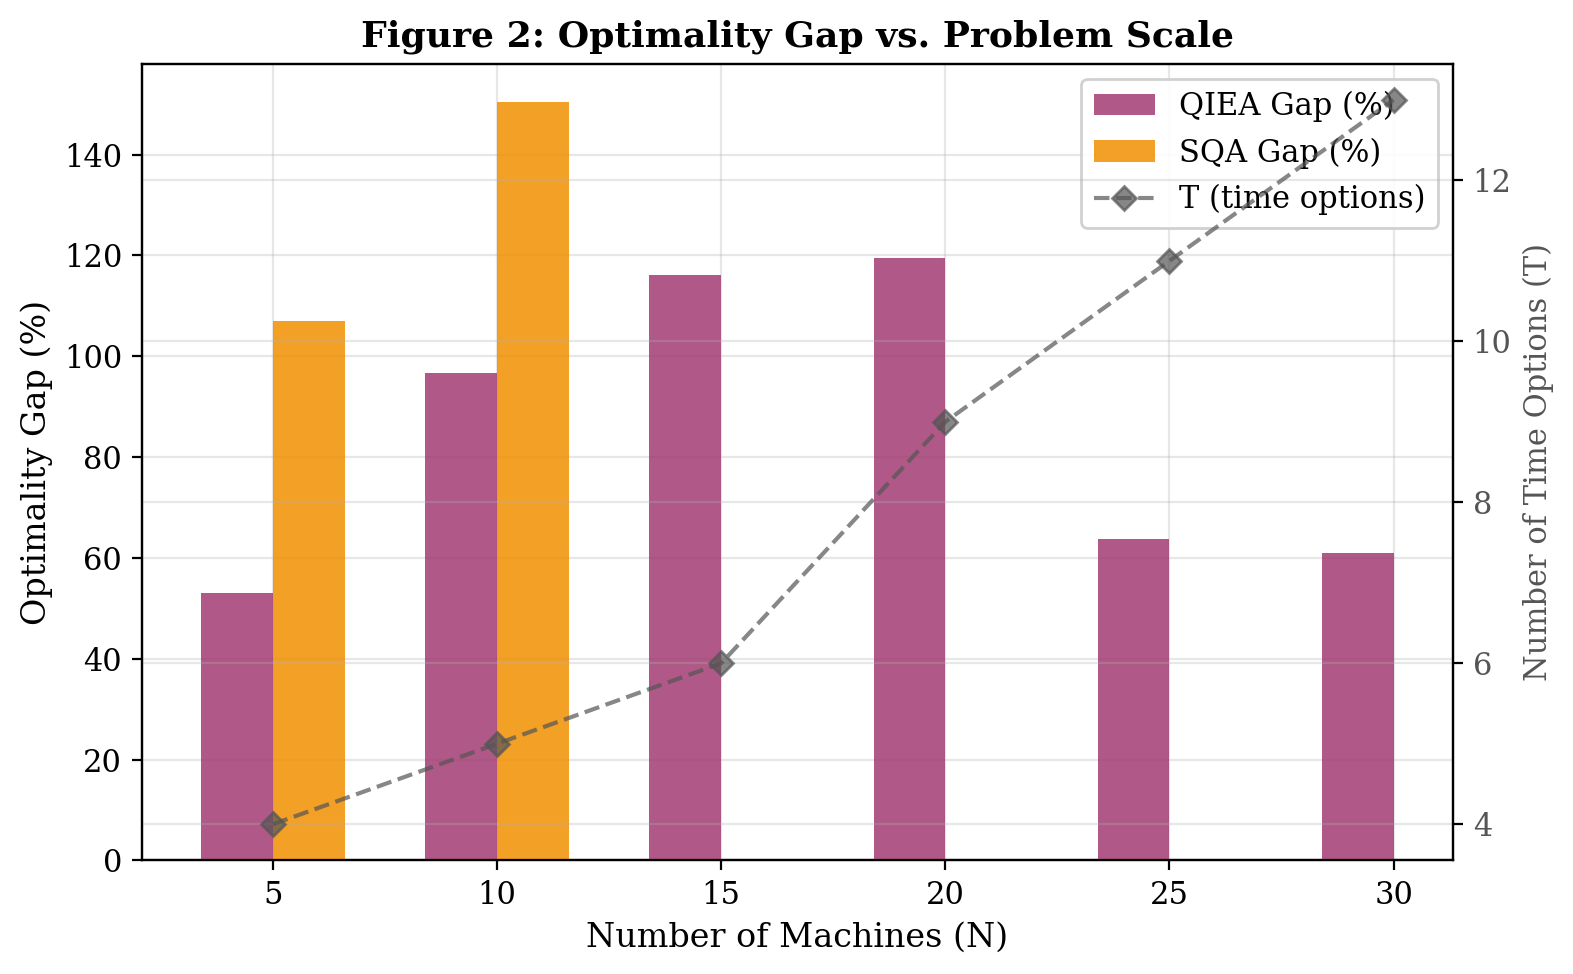
\includegraphics[width=\textwidth]{figures/images/fig2_optimality_gap.png}
        \caption{Optimality gap relative to MILP baseline across fleet sizes.}
        \label{fig:gap_optimality}
    \end{subfigure}

    \caption{Scaling benchmark results: (a) total scheduling cost and (b) optimality gap versus MILP baseline as fleet size $N$ increases.}
    \label{fig:scaling-optimality}
\end{figure}

The per-machine average cost reveals an important trend:

\begin{table}[htbp]
\centering
\caption{Per-Machine Cost Comparison (MILP vs QIEA)}
\label{tab:per_mac}
\renewcommand{\arraystretch}{1.2}

\begin{tabularx}{0.8\textwidth}{
c c c c
}
\toprule
\textbf{N} & \textbf{MILP per Machine} & \textbf{QIEA per Machine} & \textbf{Ratio} \\
\midrule

5  & 106.33 & 162.65 & 1.53x \\
10 & 130.31 & 256.31 & 1.97x \\
15 & 145.36 & 314.21 & 2.16x \\
20 & 161.08 & 353.54 & 2.19x \\
25 & 179.60 & 293.93 & 1.64x \\
30 & 213.79 & 343.92 & 1.61x \\

\bottomrule
\end{tabularx}

\end{table}

\begin{figure}[htbp]
    \centering
    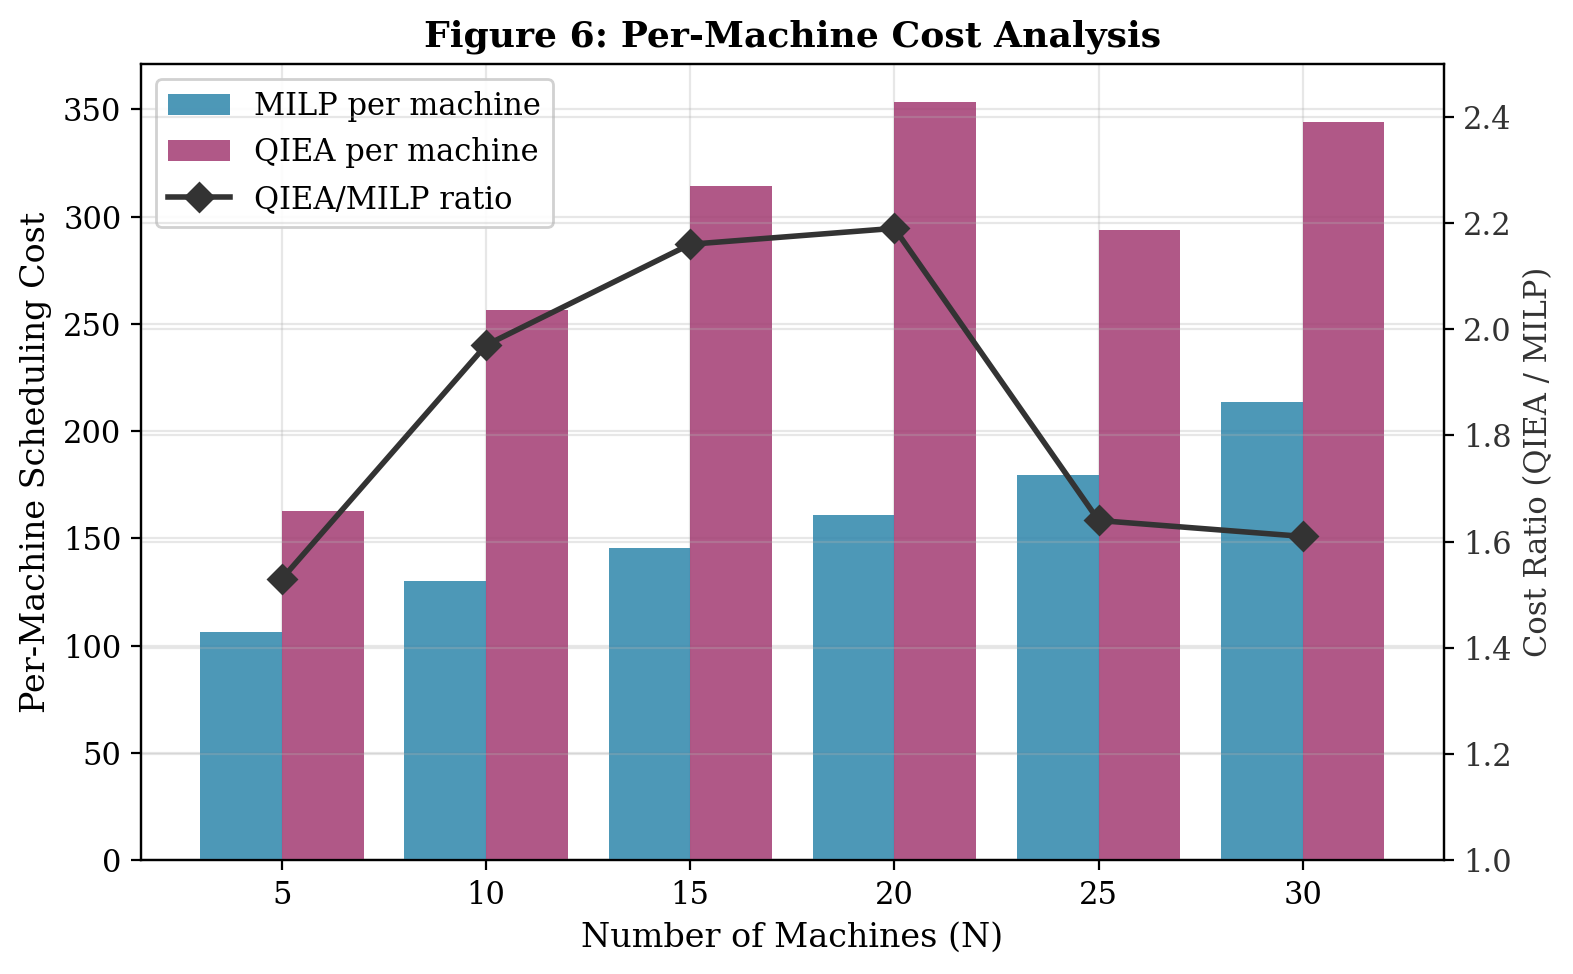
\includegraphics[width=1\textwidth]{figures/images/fig6_per_machine_cost.png}
    \caption{Per-machine average cost comparison between MILP optimal baseline and QIEA heuristic across fleet sizes $N=5$ to $N=30$.}
    \label{fig:machine-cost}
\end{figure}

\subsection{IBM Quantum Hardware Results}
Table 4 summarizes the QAOA scaling study executed on the IBM Heron r2 processor $(ibm_fez$, 156 qubits) with p = 4 QAOA layers and 4,096 measurement shots per run.
